% This LaTeX file contains your written lab questions.  You may answer these
% questions just by inserting your answer into this document.
%
% If you're unfamiliar with LaTeX, see the document LearningLaTeX.tex in this
% same directory.  It contains a brief explanation and a few snippets of LaTeX
% code to get you started; in fact, it should have everything you need to
% complete this assignment.
%
% Also see the example file in examples/week-04/bigO.tex
\documentclass{article}

\usepackage{amsmath}
\usepackage{amssymb}
\usepackage{amsthm}
\usepackage{graphicx}

\begin{document}

    \section{QuickSort}

    See the source code file \texttt{quickSort.cpp} and the tests given in
    \texttt{tests.cpp}.

    \section{Big-O Proofs}

    \vspace{2mm}
    \noindent {\large\textbf{Problem 1.}} Show that $5n^3+n^2+4$ is $O(n^3)$.\\

    %
    $\exists \; c=10, \; n_0=1$ such that $\forall \; n \geq n_0, \; f(n) \leq c(n^3)$.\\ \\
    We know that the following inequalities hold:\\ \\
    $5n^3 \leq 5n^3$,\\ \\
    $n^2 \leq n^3$,\\ \\
    $4 \leq 4n^3$.\\ \\
    Adding up the values on the left-hand side and the right-hand side of the above inequalities,
    we get the following inequality: \\ \\
    $5n^3+n^2+4 \leq 5n^3+n^3+4n^3$.\\ \\
    Hence, $5n^3+n^2+4 \leq 10n^3$, and we have proved that $5n^3+n^2+4$ is $O(n^3)$.\\

    \vspace{1cm}
    \noindent {\large\textbf{Problem 2.}} Show that $2n^4-3n^2+n$ is $O(n^4)$. \\

     %
     $\exists \; c=6, \; n_0=1$ such that $\forall \; n \geq n_0, \; f(n) \leq c(n^4)$.\\ \\
     We know that the following inequalities hold:\\ \\
     $2n^4 \leq 2n^4$,\\ \\
     $-3n^2 \leq 3n^4$,\\ \\
     $n \leq n^4$.\\ \\
     Adding up the values on the left-hand side and the right-hand side of the above inequalities,
     we get the following inequality: \\
     $2n^4-3n^2+n \leq 2n^4+3n^4+n^4$.\\ \\
     Hence, $2n^4-3n^2+n \leq 6n^4$, and we have proved that $2n^4-3n^2+n$ is $O(n^4)$.\\
 
    \vspace{1cm}
    \section{Mystery Functions}

    Function A is $O(n)$ because the for loop goes through $\frac{n}{2}$ times. \\ \\
    Function B is $O(n^2)$ because it is a nested for loop that has a runtime of $n*n$, which is $n^2$. \\ \\
    Function C is $O(n* \log n)$ because the for loop outside goes $n$ times, and the while loop's condition means that we go through $\log_{2} n$ times. \\ \\
    Function D is $O(n^4)$ because it is a nested for loop that has a runtime of $n^2*n^2$, which is $n^4$. \\ \\
    Function E is $O(4n)$ because it is a nested for loop that has a runtime of $n*4$. \\ \\
    Function F is $O(n^3)$ because the for loop goes through $n^3$ times. 
    
    \begin{itemize}
        \item \textbf{\textit{The mystery functions A-E in sorted order from fastest to slowest are}}: \\ \\
              A \; E \; C \; B \; F \; D
    \end{itemize}

    \begin{itemize}
        \item \textbf{\textit{Overall Matching Results}}: \\ \\
            A matches 3, B matches 5, C matches 4, D matches 6, E matches 2, F matches 1.
        \item \textbf{\textit{Explanation}}: \\ \\ 
            \textbf{fnD matches mystery function 6.} \\ \\
            Reason: when we first graph all 6 functions altogether on one graph within $10 \leq n \leq 100$, it is obvious that function 6 is the slowest.
            And according to our sorted order above, function D is the slowest, so these two match. \\ \\ 
            Graph to support the claim: 
            \begin{center}
                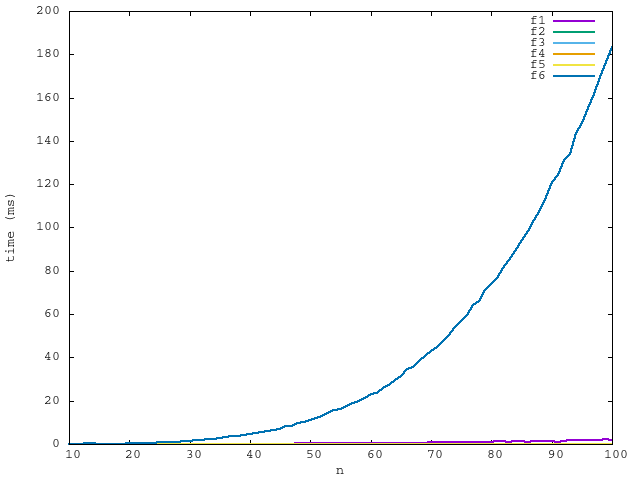
\includegraphics[width=0.8\textwidth]{f_all_10_100}
            \end{center}
    
            \textbf{fnF matches mystery function 1.} \\ \\
            Reason: now we know that function 6 corresponds to fnD, so we can do the comparison between function 1-5. If we graph these 5 functions altogether on 
            one graph within $10 \leq n \leq 100$, it is obvious that function 1 is the slowest amongst the five functions, which corresponds to function F. \\ \\
            Graph to support the claim: 
            \begin{center}
                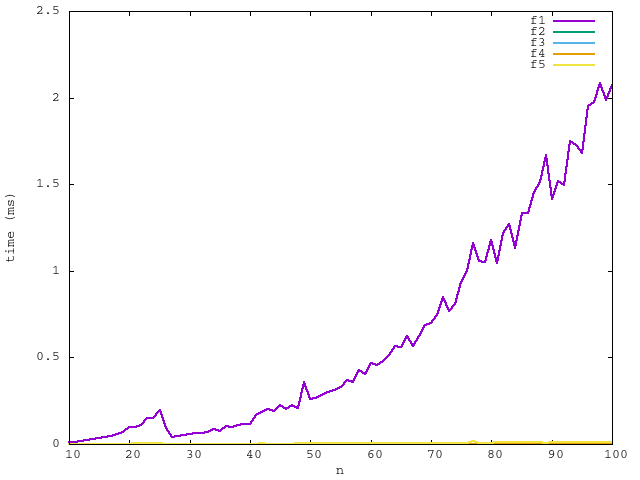
\includegraphics[width=0.8\textwidth]{f1_to_f5_10_100}
            \end{center} 
            \vspace{10cm}
            \textbf{fnB matches mystery function 5.} \\ \\
            Reason: now we are left with functions 2-5. Putting these 4 functions altogether on one graph within $200 \leq n \leq 500$, it is obvious that function 5 is the
            slowest amongst these four, and hence function 5 corresponds to function B according to the sorting order above. \\ \\
            
            \textbf{fnC matches mystery function 4.} \\ \\
            Reason: since function 1, 5, 6 have already found the correct matches. We are then left with functions 2, 3, 4. Graphing these altogether on one graph 
            within $800 \leq n \leq 1000$, it is obvious that function 4 is the slowest, which correponds to function C according to the sorting order above. \\ \\
            
            \textbf{fnE matches mystery function 2.} \\ \\
            Reason: now we are only left with function 2 and function 3. Graphing these two altogether within $1500 \leq n \leq 3000$, we see that function 2 is slower
            compared to function 3, so 3 corresponds to function E. \\ \\
            
            \textbf{fnA matches mystery function 3.} \\ \\
            Reason: we are left with only one option - function 3, which is the fastest and hence corresponds to function A.         
    \end{itemize}
\end{document}
